\documentclass{standalone}
\usepackage{pgf,tikz}
\usetikzlibrary{calc}

\begin{document}

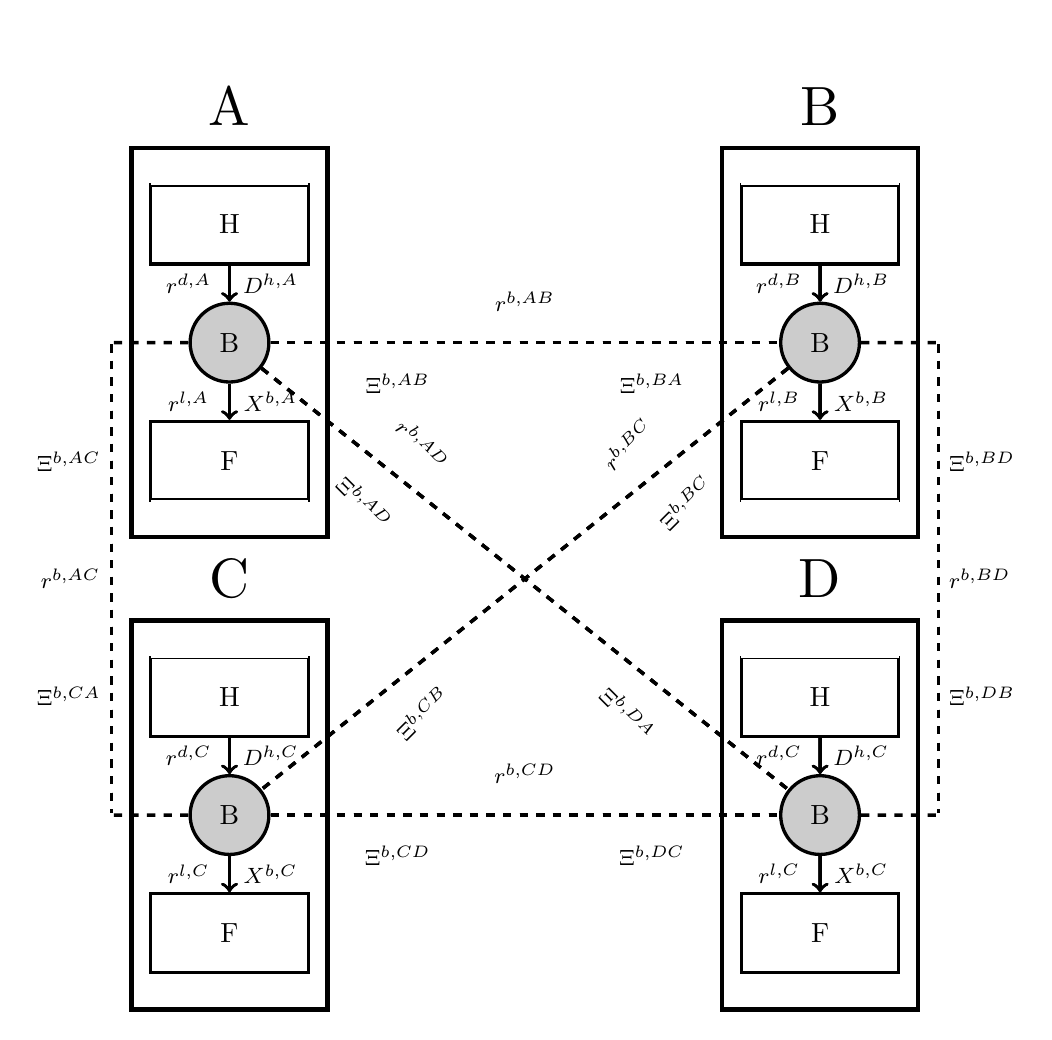
\begin{tikzpicture}[scale=0.75,
every node/.style={draw,solid,fill=black!20, very thick, minimum size = 1cm}]

\node [fill=white,minimum width=2cm] at (0,4) (H_A) {H};
\node [circle] at (0,2) (B_A) {B};
\node [fill=white,minimum width=2cm] at (0,0) (F_A) {F};

               
\node [fill=white,minimum width=2cm] at (10,4) (H_B) {H};
\node [circle] at (10,2) (B_B) {B};
\node [fill=white,minimum width=2cm] at (10,0) (F_B) {F};


\node [fill=white,minimum width=2cm] at (0,-4) (H_C) {H};
\node [circle] at (0,-6) (B_C) {B};
\node [fill=white,minimum width=2cm] at (0,-8) (F_C) {F};

               
\node [fill=white,minimum width=2cm] at (10,-4) (H_D) {H};
\node [circle] at (10,-6) (B_D) {B};
\node [fill=white,minimum width=2cm] at (10,-8) (F_D) {F};

\node [draw = none,fill=white,minimum size = 0pt,inner sep=0pt] at (-2,2) (conn_1) {};
\node [draw = none,fill=white,minimum size = 0pt,inner sep=0pt] at (-2,-6) (conn_2) {};

\node [draw = none,fill=white,minimum size = 0pt,inner sep=0pt] at (12,2) (conn_3) {};
\node [draw = none,fill=white,minimum size = 0pt,inner sep=0pt] at (12,-6) (conn_4) {};

\node [draw=none,fill=white,scale=2] at (0,6) (label_A) {A};
\node [draw=none,fill=white,scale=2] at (10,6) (label_B) {B};
\node [draw=none,fill=white,scale=2] at (0,-2) (label_C) {C};
\node [draw=none,fill=white,scale=2] at (10,-2) (label_D) {D};

%///////////////////////////////////////////
% Intra-regional flows - Deposits and credit
%//////////////////////////////////////////

% A

\draw[->, very thick] (H_A) -- (B_A) node [draw=none,fill=none,font=\footnotesize,midway,left] {$r^{d,A}$};
\draw[->, very thick] (H_A) -- (B_A) node [draw=none,fill=none,font=\footnotesize,midway,right] {$D^{h,A}$};
\draw[->, very thick] (B_A) -- (F_A) node [draw=none,fill=none,font=\footnotesize,midway,left] {$r^{l,A}$};
    \draw[->, very thick] (B_A) -- (F_A) node [draw=none,fill=none,font=\footnotesize,midway,right] {$X^{b,A}$};
    
% B
    
\draw[->, very thick] (H_B) -- (B_B) node [draw=none,fill=none,font=\footnotesize,midway,left] {$r^{d,B}$};
\draw[->, very thick] (H_B) -- (B_B) node [draw=none,fill=none,font=\footnotesize,midway,right] {$D^{h,B}$};
\draw[->, very thick] (B_B) -- (F_B) node [draw=none,fill=none,font=\footnotesize,midway,left] {$r^{l,B}$};
\draw[->, very thick] (B_B) -- (F_B) node [draw=none,fill=none,font=\footnotesize,midway,right] {$X^{b,B}$};

% C
    
\draw[->, very thick] (H_C) -- (B_C) node [draw=none,fill=none,font=\footnotesize,midway,left] {$r^{d,C}$};
\draw[->, very thick] (H_C) -- (B_C) node [draw=none,fill=none,font=\footnotesize,midway,right] {$D^{h,C}$};
\draw[->, very thick] (B_C) -- (F_C) node [draw=none,fill=none,font=\footnotesize,midway,left] {$r^{l,C}$};
\draw[->, very thick] (B_C) -- (F_C) node [draw=none,fill=none,font=\footnotesize,midway,right] {$X^{b,C}$};

% D
    
\draw[->, very thick] (H_D) -- (B_D) node [draw=none,fill=none,font=\footnotesize,midway,left] {$r^{d,C}$};
\draw[->, very thick] (H_D) -- (B_D) node [draw=none,fill=none,font=\footnotesize,midway,right] {$D^{h,C}$};
\draw[->, very thick] (B_D) -- (F_D) node [draw=none,fill=none,font=\footnotesize,midway,left] {$r^{l,C}$};
\draw[->, very thick] (B_D) -- (F_D) node [draw=none,fill=none,font=\footnotesize,midway,right] {$X^{b,C}$};
  
%///////////////////////////////////////////
% Inter-regional flows - Interbank exposures
%//////////////////////////////////////////

% A-B
    
\draw[dashed, very thick] (B_A) -- (B_B) node [draw=none,fill=none,font=\footnotesize,midway,above] {$r^{b,AB}$};
\draw[dashed, very thick] (B_A) -- (B_B) node [draw=none,fill=none,font=\footnotesize,near start,below] {$\Xi^{b,AB}$};
\draw[dashed, very thick] (B_A) -- (B_B) node [draw=none,fill=none,font=\footnotesize,near end,below] {$\Xi^{b,BA}$};

% A-C

\draw[dashed, very thick] (conn_1) -- (conn_2) node [draw=none,fill=none,font=\footnotesize,midway,left] {$r^{b,AC}$};
\draw[dashed, very thick] (conn_1) -- (conn_2) node [draw=none,fill=none,font=\footnotesize,near start,left] {$\Xi^{b,AC}$};
\draw[dashed, very thick] (conn_1) -- (conn_2) node [draw=none,fill=none,font=\footnotesize,near end,left] {$\Xi^{b,CA}$};

\draw[dashed, very thick] (B_A) -- (conn_1);
\draw[dashed, very thick] (B_C) -- (conn_2);

% B-D

\draw[dashed, very thick] (conn_3) -- (conn_4) node [draw=none,fill=none,font=\footnotesize,midway,right] {$r^{b,BD}$};
\draw[dashed, very thick] (conn_3) -- (conn_4) node [draw=none,fill=none,font=\footnotesize,near start,right] {$\Xi^{b,BD}$};
\draw[dashed, very thick] (conn_3) -- (conn_4) node [draw=none,fill=none,font=\footnotesize,near end,right] {$\Xi^{b,DB}$};

\draw[dashed, very thick] (B_B) -- (conn_3);
\draw[dashed, very thick] (B_D) -- (conn_4);

% C-D

\draw[dashed, very thick] (B_C) -- (B_D) node [draw=none,fill=none,font=\footnotesize,midway,above] {$r^{b,CD}$};
\draw[dashed, very thick] (B_C) -- (B_D) node [draw=none,fill=none,font=\footnotesize,near start,below] {$\Xi^{b,CD}$};
\draw[dashed, very thick] (B_C) -- (B_D) node [draw=none,fill=none,font=\footnotesize,near end,below] {$\Xi^{b,DC}$};

% A-D

\draw[dashed, very thick] (B_A) -- (B_D) node [draw=none,fill=none,font=\footnotesize,near start,above,rotate=-45] {$r^{b,AD}$};
\draw[dashed, very thick] (B_A) -- (B_D) node [draw=none,fill=none,font=\footnotesize,near start,below,rotate=-45] {$\Xi^{b,AD}$};
\draw[dashed, very thick] (B_A) -- (B_D) node [draw=none,fill=none,font=\footnotesize,near end,below,rotate=-45] {$\Xi^{b,DA}$};

% B-C

\draw[dashed, very thick] (B_B) -- (B_C) node [draw=none,fill=none,font=\footnotesize,near start,above,rotate=45] {$r^{b,BC}$};
\draw[dashed, very thick] (B_B) -- (B_C) node [draw=none,fill=none,font=\footnotesize,near start,below,rotate=45] {$\Xi^{b,BC}$};
\draw[dashed, very thick] (B_B) -- (B_C) node [draw=none,fill=none,font=\footnotesize,near end,below,rotate=45] {$\Xi^{b,CB}$};


% Regions
         	
\draw[black,ultra thick,solid] ($(H_A.north west)+(-0.3,0.6)$)  rectangle ($(F_A.south east)+(0.3,-0.6)$);

\draw[black,ultra thick,solid] ($(H_B.north west)+(-0.3,0.6)$)  rectangle ($(F_B.south east)+(0.3,-0.6)$);

\draw[black,ultra thick,solid] ($(H_C.north west)+(-0.3,0.6)$)  rectangle ($(F_C.south east)+(0.3,-0.6)$);

\draw[black,ultra thick,solid] ($(H_D.north west)+(-0.3,0.6)$)  rectangle ($(F_D.south east)+(0.3,-0.6)$);
                  
\end{tikzpicture}

\end{document}